\documentclass[14pt]{extarticle}

\usepackage[utf8]{inputenc}
\usepackage[T2A,T1]{fontenc}
\usepackage[russian]{babel}
\usepackage[a4paper,lmargin=3cm,rmargin=2cm,tmargin=2cm,bmargin=2cm]{geometry}
\usepackage[ddmmyyyy]{datetime}
\usepackage{indentfirst}
\usepackage{hyperref}
\usepackage{graphicx}
\graphicspath{{./images/}}

\usepackage{minted}

\usepackage{titlesec}
\titleformat{\section}{\normalfont\bfseries\centering}{\thesection}{1em}{}
\titleformat{\subsection}{\normalfont\bfseries}{\thesubsection}{1em}{}
\usepackage{setspace}
\singlespacing
%\onehalfspacing
%\doublespacing
\setlength{\parindent}{1.25cm}
\let\oldsection\section
\renewcommand\section{\clearpage\oldsection}

\usepackage[backend=biber]{biblatex}
\addbibresource{~/texdoc/bibl.bib}
\input{~/texdoc/unibind.tex}

\usepackage{pgf}
\usepackage{tikz}
\usetikzlibrary{arrows,automata}
\usetikzlibrary{positioning}

\tikzset{
	state/.style={
		rectangle,
		draw=black, very thick,
		anchor=west, align=left,
		text width=6cm,
	},
}
\usepackage{csquotes}

\usepackage{multirow} %\multirow{NUMBER_OF_ROWS}{WIDTH}{CONTENT}
% \multicolumn{NUMBER_OF_COLUMNS}{ALIGNMENT}{CONTENT}

\begin{document}
\unititle
{\klgtu}
{\fapu}
{\suvt}
{Лабораторная Работа}
{По дисциплине: «Сетевые информационные технологии и программирование» \par Работа 6}
{Доцент}
{Ломакина Г.В.}
{ст. гр. 18-ВТ}
{Поляков Л.Д.}

\tableofcontents

\section{Задание}

\begin{itemize}
	\item Задание 1
	Подготовить реферат по следующим  вопросам: 
	\begin{enumerate}
		\item Классификация WEB-сайтов (одинаковый для всех);
		\item Этапы разработки WEB-сайтов (одинаковый для всех);
		\item Оптимизация сайта.
	\end{enumerate}

	\item Задание 2
	 Выполнить установку локального сервера и выбранной CMS-системы на свой компьютер.
	\item Задание 3
	 Используя установленную CMS-систему, создать сайт, содержащий 5-6 страниц.
\end{itemize}

\section{Ход Разработки}

\begin{figure}[ht]
    \centering
	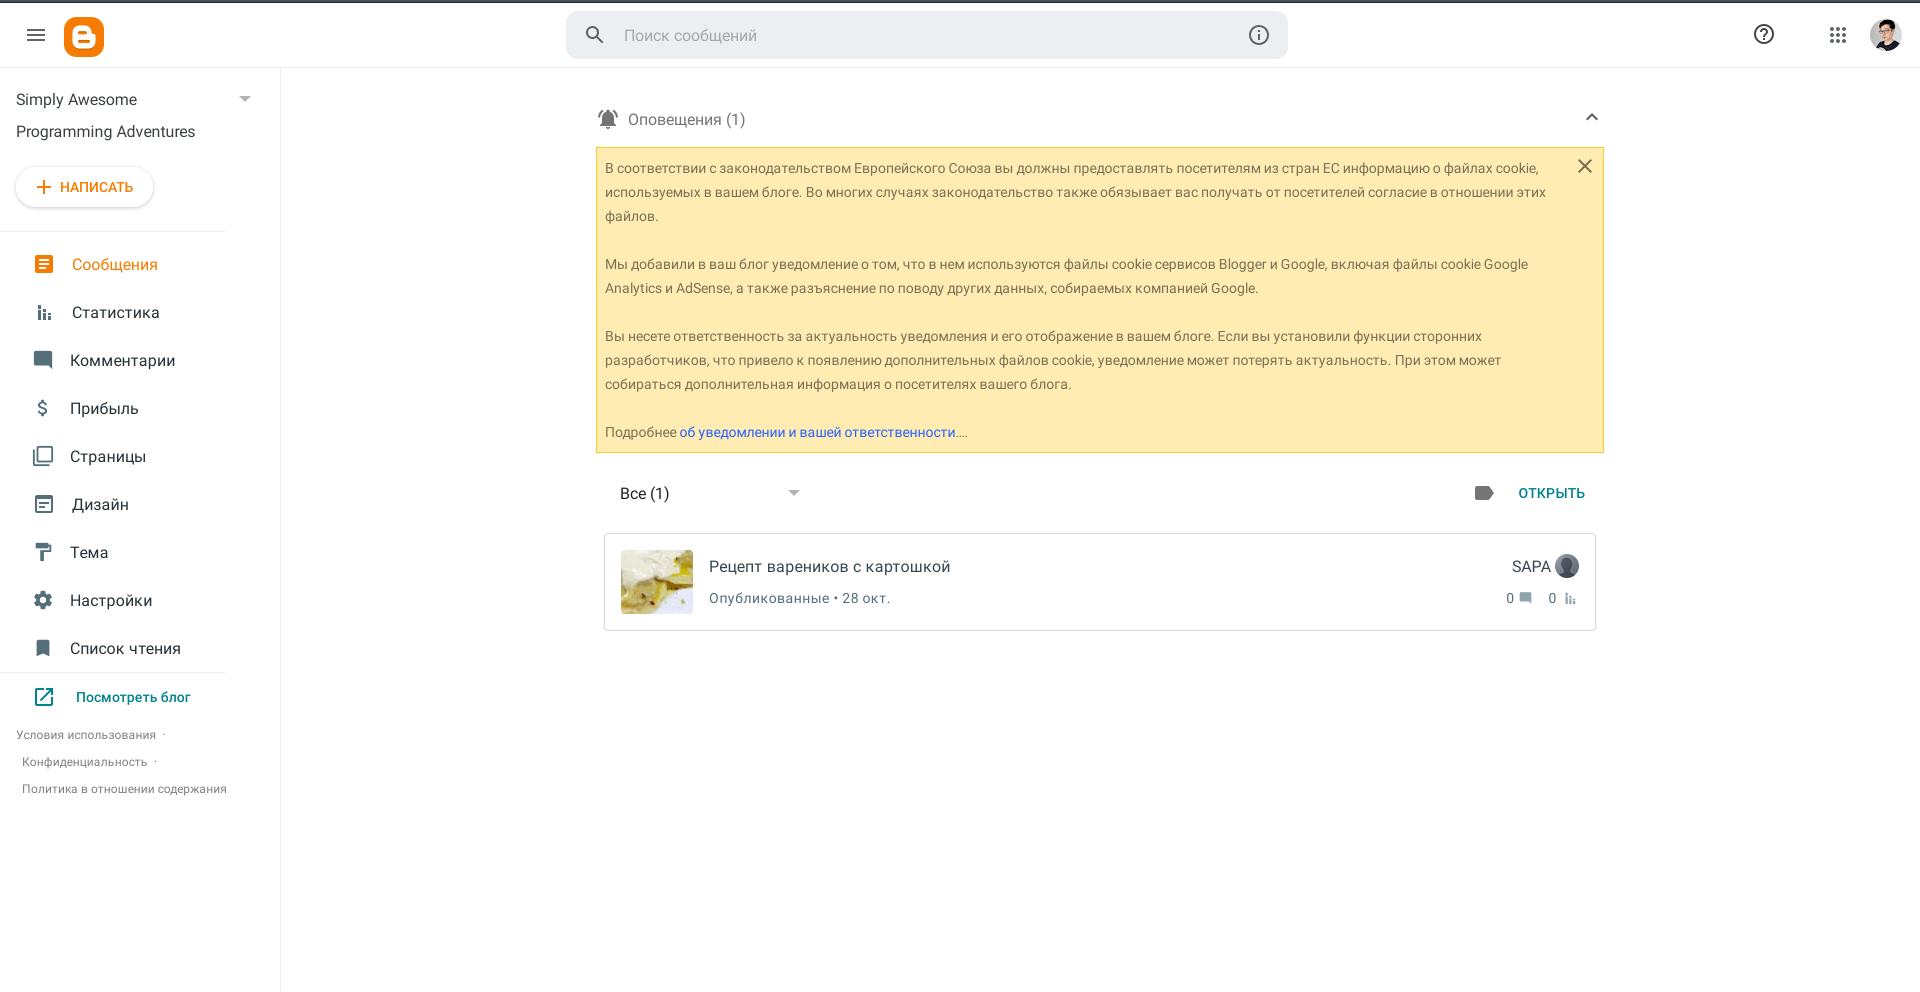
\includegraphics[width=0.9\textwidth, angle=0]{2021-12-12_21-10}
    \caption{Заход на страницу Blogger.com и создание блога \#1}
    \label{fig:html1}
\end{figure}


\end{document}
